\section{System Description}
The system described here is designed to run on Linux and its operability has been confirmed on Ubuntu.
%
\subsection{Basic Terminology}
A \term{node}---as it relates to our system---is a single computer that can operate independently.
A \term{process} is an instance of a program that is being executed; each process contains the program code and the memory in use by the current execution.
%
%\subsection{Bitmaps}
%A bitmap index is an indexing method often compares
%
\subsection{Client}
Our system's \term{client} is a database management system (DBMS).
A DBMS interfaces with our system through two actions:
\code{PUT} which adds data to the system (or updates existing data), and
\code{QUERY} which requests the results of a given query on the index.
In production, the DBMS could be a full-featured product like SQLite, but we created a faux DBMS that provided fine-grained control for our testing.
%
\subsection{System Structure}
The two most established structures for a distributed system are the master-slave model and the peer-to-peer model; in both cases, let us assume we have \(N\) total nodes.
In both models, a client (be it a person, another system, etc.) makes a request of the system and will expect some sort of response (a result, an acknowledgment, etc.).
In the peer-to-peer model each of the \(N\) peers can accept requests and then delegate work to their peers.
Once the request has been satisfied, whichever peer has the final result will return the result to the client.
In the master-slave model there exits a single ``master'' node and \(N - 1 = n\) ``slave'' nodes.
The master node accepts requests and then delegates the work to the slaves which return results to the master which will in turn return the final result to the client.
We chose to structure our system using the master-slave model instead of a peer-to-peer model because it is a very intuitive way of structuring the query problem.
Further, when distributing data to the slaves we have chosen to use a replication factor of two---i.e., each piece of data is stored on two separate nodes.
%
\subsection{Communication}
Distributed systems require additional methods of communication beyond those used in single-process or even single-node systems.
Communication between nodes was accomplished using remote procedure calls (RPCs). An RPC is simply a function call
from one process to another \cite{tanenbaum1994}.
RPCs are a method of simplifying communication between nodes by hiding the networking details and instead allowing developers to make function calls between nodes.
This helps to make the source code more readable and avoid mistakes in manually opening and closing network connections.

%
\subsection{Bitmap Compression}
In order to perform the necessary bitmap operations (\code{AND}s and \code{OR}s), we utilized a Bitmap Engine which had been developed by several students under the direction of Professor David Chiu.
The Bitmap Engine has implemented three compression and query methods: Byte aligned Bitmap Code (BBC), Word aligned Hybrid Code (WAH), and Variable aligned Length Code (VAL).
Each of these three compression and query methods provides substantial benefits over the use of uncompressed bitmap vectors.
Of the three, we chose to use WAH as it has been shown to be faster than BBC and it has a simpler formatting than VAL.
WAH allows compression of vectors such that all information the vector gives
is encoded, allows compressed vectors to be queried. A complete description of
WAH is given by \cite{}.
%
\subsection{Consistent Hashing}
We use an algorithm known as consistent hashing, introduced by Karger et al \cite{karger1997} to determine which two machines a given vector is located, or
should be located if the identifier is new to the system.
Conceptually, consistent hashing can be understood as follows. Each slave machine is assigned a point on a circle, where each point
corresponds to a value between $0$ and $2^{64}-1.$ The point for a machine with identifier $i$ is calculated as $h(i):=\textsc{SHA1}(i)\bmod 2^{64}.$ To determine which machines (should) contain a given vector $k$, determine the point $h(k)$, and from that point walk clockwise until reaching a machine node. Keep walking until reaching the next node, and return that node (the \emph{backup} node) and the previous (\emph{primary}) node. The process is depicted in Figure 1.
\begin{figure}
    \centering
    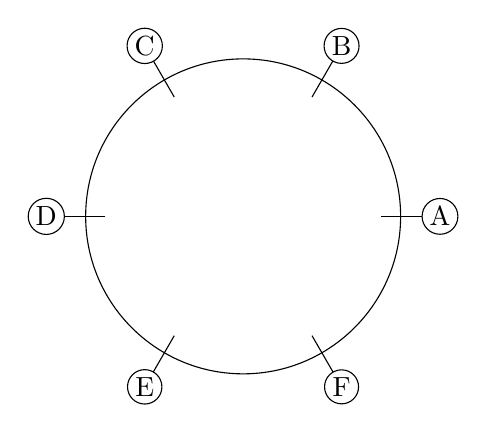
\begin{tikzpicture}
    \draw (0,0) circle (2);
    \draw (0:1.75) -- (0:2.5) node [draw, shape=circle, inner sep=1, fill=white, text=black] {A};
    \draw (60:1.75) -- (60:2.5) node [draw, shape=circle, inner sep=1, fill=white, text=black] {B};
    \draw (120:1.75) -- (120:2.5) node [draw, shape=circle, inner sep=1, fill=white, text=black] {C};
    \draw (180:1.75) -- (180:2.5) node [draw, shape=circle, inner sep=1, fill=white, text=black] {D};
    \draw (240:1.75) -- (240:2.5) node [draw, shape=circle, inner sep=1, fill=white, text=black] {E};
    \draw (300:1.75) -- (300:2.5) node [draw, shape=circle, inner sep=1, fill=white, text=black] {F};
\end{tikzpicture}

    \caption{Visualization of Ring Consistent Hashing}
\end{figure}
In our system, the consistent hashing strucure is maintained as a red-black tree, and the process of determining the next node is given by the $\textsc{Tree-Successor}$ algorithm. When the system is initialized,
each machine identifier (a nonnegative integer) is inserted into the tree. Each node is identified according to $h(i)$ as the field $hash$. Each node also has pointers to its left child, right child, and parent, $left, right$ and $p$ respectively.
A tree also has a ``null'' node, $tree.nil$, as a parent or child if it doesn't have one.
\begin{algorithm}
  \Procedure{Tree-Successor}{$tree,key$}
    \begin{algorithmic}
      \State{$digest\gets h(key)$}
      \If{$digest\geq\textsc{Tree-Max}(tree).hash$}\\
          \Return{$\textsc{Tree-Min}(tree)$}
      \Else\\
        \Return{$\textsc{Recur-Succ}(tree,tree.root,\\tree.root,key)$}
      \EndIf
    \end{algorithmic}
\caption{Successor node}
\end{algorithm}
$\textsc{Tree-Min},\textsc{Tree-Max}$ are given in CLRS.
\begin{algorithm}
  \Procedure{Recur-Succ}{$t,root,succ,key$}
   \begin{algorithmic}
     \If{$root = t.nil$}\\
      \Return $succ$
     \EndIf
     \If{$key=root.hash$}%\Comment{Find leftmost node of right subtree}
      \State{$succ\gets root.right$}
      \If{$succ = t.nil$}
       \State{$succ\gets root$}
       \While{$succ.p\neq t.nil\land succ.hash<key$}
        \State{$succ \gets succ.p$}
       \EndWhile
      \Else
       \While{$succ.left \neq t.nil$}
        \State{$succ \gets succ.left$}
        \EndWhile
      \EndIf
      \Return {$succ$}
    \EndIf
    \If{$root.hash > key$}\\
        \Return{$\textsc{Recur-Succ}(t, root.left, root, key)$}
    \EndIf
    \Else\\
      \Return{$\textsc{Recur-Succ}(t, root.right, succ, key)$}
    \EndElse
   \end{algorithmic}
\caption{Recursively determine successor node}
\end{algorithm}

The algorithm for consisent hashing is as follows.
\begin{algorithm}
  \Procedure{Consistent-Hash}{$key,tree$}
    \begin{algorithmic}
      \State{$m_0 \gets \textsc{Tree-Successor}(tree, key)$}
      \State{$m_1 \gets \textsc{Tree-Successor}(tree, m_0.id)$}\\
      \Return{$\{m_0,m_1\}$}
    \end{algorithmic}
\caption{Consistent Hashing}
\end{algorithm}
\subsection{Fault Tolerance}
%
The primary reason for using consistent hashing is for fault tolerance. To ensure
that each slave node is still online, while waiting for messages from the DBMS
the master pings each slave. If it doesn't hear back from a slave after one second,
it assumes that slave is out of commission, and reallocates the vectors using
$\textsc{Reallocate}$. To each node in the tree we store the set of vectors that
map to this machine, specifically for this purpose.
\begin{algorithm}
  \Procedure{Reallocate}{$tree, slave$}
    \begin{algorithmic}
      \State{$pred\gets\textsc{Tree-Predecessor}(tree, slave)$}
      \State{$succ\gets\textsc{Tree-Successor}(tree, slave)$}
      \State{$second\_succ\gets\textsc{Tree-Successor}(tree, succ)$}
      \ForAll{$v\in pred.vectors$}
        \State{$\textsc{Send-Vector}(pred, v.id, succ)$}
      \EndFor
      \ForAll{$w\in slave.vectors$}
        \State{$\textsc{Send-Vector}(succ, w.id, second\_succ)$}
      \EndFor
      \State{$succ.vectors\gets succ.vectors\cup slave.vectors$}
      \State{$\textsc{RB-Delete}(tree,slave)$}
    \end{algorithmic}
    \caption{Reallocation}
\end{algorithm}
$\textsc{Tree-Predecessor},\textsc{Tree-Successor},$ and $\textsc{RB-Delete}$ are given
in CLRS. $\textsc{Send-Vector}(s_1,k,s_2)$ is an RPC that orders slave $s_1$ to send
$s_2$ vector $k$. Because we used consistent hashing, we know that the failed slave's
backup vectors are the primary vectors of its predecessor. The successor must
now maintain copies of the predecessor's vectors, so the master tells the predecessor to communicate
its primary vectors to the successor.
Likewise, since the successor node now holds the slave's primary vectors alongside
its own, it must send the slave's primary vectors to its successor as a backup.
Consistent hashing is preferable to using a hash-mod-n or round-robin technique
because potentially every every single vector would have to be remapped,
requiring significantly more messages and more nodes involved than the ones
used in $\textsc{Reallocate}$ to reconfigure the system. This is because for
hash-mod-n and round robin, algorithms whose hash function modulus is
the number of machines, when a slave node is removed, the primary locations
of potentially every vector changes, thus requiring us to remap every
single vector \cite{kleppman2017}. While hash-mod-n requires $O(K)$ remappings,
where $K$ is the number of keys, consistent hashing only requires $O(K/n)$,
where $n$ is the number of slaves \cite{karger1997}.
%
\subsection{Consistency}
After we have decided \emph{where} to store data, we needed a method of ensuring that the data actually arrived at each node it was suppose to.
To do this, we implemented a system called Two-Phase Commit (TPC) which ensures data consistency.
It does this by checking that both slaves are available: if so, the data is sent to both, if either is unavailable, the unavailable node is handled and the process is restarted.
%
\subsection{Queries}
Our system is designed to handle range queries. An example range query is
\texttt{R:[0,3]\&[5,7]}. Such a query might correspond to a range query in SQL.
This query requires the following steps:
$$
v\gets v_0 \lor v_1 \lor v_2 \lor v_3 $$ $$
w\gets v_5 \lor v_6 \lor v_7 $$ $$
\texttt{return }  v \land w
$$
To carry out the query, we first create a plan that tells us which slave nodes
to visit.
\subsection{Query Planning}
%\caption{Algorithm to plan query}\\
The input value $Ranges$ is an ordered set of tuples $\{\{v_0,v_1\},\{v_1,v_2\},\ldots,\{v_n,v_m\}\}$ where $v_i\leq v_j$ and $0\leq i\leq j\leq n\leq m$, and each $v_i$ is a vector identifier, and $tree$ is the red-black tree used in
consistent hashing to determine which two machines contain a given vector identifier.

\begin{algorithm}
  \Procedure{Range-Query-Plan}{$Ranges, tree$}
    \begin{algorithmic}
        \State{$swap \gets $  false}% \Comment{Used to choose the first or second result from CH.}
        \State{$paths \gets \emptyset$}
            \ForAll{$r \in\emph{Ranges}$}
                \State{$subpaths \gets \emptyset$}
                \For{$k \gets r_0,r_1$}
                  \State{$machines \gets \textsc{Consistent-Hash}(k,tree)$}%\Comment{A set containing the two machines this vector is on.}
                  \State{$tuple \gets \emptyset$}
                  \If{$swap$}
                    \State{$tuple \gets tuple \cup \{machines_0\}$}
                  \Else
                    \State{$tuple \gets tuple \cup \{machines_1\}$}
                  \EndIf
                  \State{$tuple \gets tuple \cup \{k\}$}
                  \State{$subpaths \gets subpaths \cup tuple$}
                \EndFor
                \State{Sort $subpaths$ on $machine.id$}
                \State{$paths \gets paths \cup subpath$}
                \State{$swap \gets \neg swap$}
          \EndFor
          \Return $paths$
    \end{algorithmic}
    \caption{Query Planning}
\end{algorithm}
Sorting is performed so that in each portion of the query, we can visit each
slave once.
%
\subsection{Query Execution}
The master node plans out the query, and has the slaves execute it.
\begin{algorithm}
  \Procedure{Range-SubQuery}{$subquery$}
    \begin{algorithmic}
      \State{$res\gets \vec{0}$}
      \ForAll{$tuple\in subquery$}
        \If{$tuple_0=self$}
          \State{$res\gets res\lor \textsc{Retrieve-Vector}(tuple_1)$}
          \State{$subquery\gets subquery\setminus\{tuple\}$}
        \Else
          \State{$res\gets res\lor tuple_0.\textsc{Range-SubQuery}(tuple_1)$}
          \State{\textbf{break}}
         \EndIf
      \Return{$res$}
    \end{algorithmic}
    \caption{Slave subquery}
\end{algorithm}

\begin{algorithm}
  \Procedure{Master-Query-Root}{$query$}
    \begin{algorithmic}
      \State{$res\gets\emptyset$}
      \ForAll{$subq\in query$}
        \State{$res\gets res\cup {subq_0}_0.\textsc{Range-SubQuery}(subq)$}
      \EndFor
      \State{$v\gets res_0$}
      \ForAll{$w\in res,w\neq v$}
        \State{$v\gets v\land w$}
      \EndFor
      \Return $v$
    \end{algorithmic}
  \caption{Master Query Root}
\end{algorithm}
\subsection{Implementation and Testing Notes}
Due to its speed and established usage in systems like ours such as Redis \cite{https://github.com/antirez/redis}, we settled on writing our system primarily in the C programming language.
In addition to C, Python 3 was used to script the production of testing data,
which we obtained from the TPC-C data repository..
Python 3 was also used in collaboration with bash to produce startup scripts that facilitated automatic testing of the system.
In order to create our RPCs, we had to specify the types of RPCs being used in the ONC+ RPC language which is an extension of the eXternal Data Representation (XDR) language developed in the mid 1980s by Sun Microsystems.
